\chapter{Project Description}

\section{General Idea}
\textit{The idea of this app is to enable a low to mid size festival organisation in a relatively simple and straight-forward manner that would be easily accessible and understandable even to non-technically educated Users.}\\

\textit{The application would be open-source, and would run on the Android OS - a native mobile app.}\\

\section{Position in the market - the competition}
\textit{Mainly, the competition consists of either high-profile professional apps, or non-native(non-mobile) apps. Thus, the point of this app is to fill that gap - it's supposed to be a native app, that's relatively simple to use, and very portable and easily deployable.}\\

\textit{This would also imply, and goes hand in hand, with the fact that the application would be easy to use and easily accessible to a wide range of people - from highly-trained professional IT Users all the way to non-IT savvy amateur/inexperienced Users.}\\

\textit{Because of the low difficulty, and relatively ad rem employability, this app would be more suitable to the lower skill level(entry to mid-level) Users, as it is likely that Pro Users would require a larger scale App for, probably, larger caliber Festivals that they deal with. With that in mind however, this app can be used as a mini, mobile device reminder version of whatever Pro tool is used for Festival organisation.}\\

\textit{In the market there is presence of both event organisation, and user-event interface apps. This app is focused on organisation, and not festival-goers. Therefore, from a marketplace standpoint, there will be no impact on the demand of the application due to the selected specialisation.}\\

\section{In-Depth Description}
\textit{Application would be used for Festival organisation - music festivals, film festivals, library events, food and alcohol festivals, parties, birthdays, and other kinds of meet-ups. By scope and complexity it would be used for smaller and medium scale Events/Festivals.}\\

\textit{The system would be run and moderated by Administrators. The system/platform would allow concurrent usage by multiple Users. These Users are: Administrators, Creators, Organisers, Workers}\\

\textit{From here on, unregistered and Users who aren't logged in will be referred to as Guests.}

	\subsection{Account Data}
	\textit{Prior to registration, Guests must fill in a Registration form. This form consists of: }
	\begin{packed_item}
		\item Username
		\item Email
		\item Password
		\item Password Verification
		\item Phone Number
		\item Name
		\item Surname
		\item Desired Role
		\begin{packed_enum}
			\item Leader
			\item Organiser
			\item Worker
		\end{packed_enum}
	\end{packed_item}

	\textit{Aside from this data, Users can also upload their Pictures online. In case they don't a default anonymous one will be used. These Profile Pictures will be put on Users' Cards that serve as Festival entrance tickets.}
	
	\textit{Users can change some of this data. Specifically, they can alter:}
	\begin{itemize}
		\item Email
		\item Password
		\item Phone Number
		\item Profile Picture
	\end{itemize}
	
	\textit{Users aren't allowed to modify their Usernames in order to prevent abuse and misuse. If Users want their Usernames, Names or Surnames changed, they can contact the Administrator, and if the appeal makes sense the Administrator can change those values for the User.}
	
	\subsection{User roles}
		\subsection{Administrators}
		\textit{Maintain and organize the platform. They curate the Creators. They have complete transparency and access to all data. They can veto and issue bans on: Festivals, Jobs, User registrations, comments, etc... Basically they have complete control over the platform.}		
		
		\subsection{Creators}
		\textit{Need to be verified by one of the Administrators. Have the ability to create and edit Festivals, as well as have complete transparency of the Festivals they have created. Can undertake certain actions regarding the details of their Festivals(and Jobs).}\\
		
		\textit{They appoint and verify Organisers. To these Organisers they assign Festivals that need to be organised - delegation of Festival planning and execution. Organisers cannot organise concurrent Festivals.}
		
		\subsection{Organiser}
		\textit{Organisers are appointed by the Creators. They manage, plan and execute Festivals on both a macro and micro/detail scale. They are appointed to Festivals by Creators.}\\
		
		\textit{They can organise multiple Festivals, and be appointed to those Festivals by multiple Creators - it is only important that none of those Festivals are concurrent.}
		
		\textit{They organise and manage Jobs and Activities that need to be done for the Festival. Jobs are performed by Workers. Organisers also have the ability to write and read comments on the Worker's walls as to better organise these Jobs.}
		
		\textit{Job and Activity management is done via Auctions. First Workers apply to these Auctions, and their entries need to be verified by the Organisers. And then the Verified Entries can compete to receive the Job Offer. Should they deem it necessary, Organisers can extend Auctions by one day.}
		
		\subsection{Worker}
		\textit{They perform Jobs and Activities. For these Jobs they first have to apply to the selection process(Auctions) during which their entries are curated by the Organisers(or eventually Administrators or Creators). Upon verification, their entries compete in order for the Worker to receive the Job Offer.}\\
		
		\textit{Some Jobs are necessary to be done by multiple Workers. Workers can specify in their Auction Entry how many more Workers would the Job require. Jobs can be done concurrently(parallelised), and Workers can perform Jobs with maximum freedom, so long as these Jobs aren't concurrent - in case they are, the system will immediately veto such entries.}
		
		\textit{Workers' accounts have certain specifics compared to other accounts. Their profiles contain:}
		\begin{packed_enum}
			\item Field of specialisation
			\item Basic account data and information
			\item Former Job information
			\item Comment section on the Worker’s profile wall – intended to allow the Worker’s co-workers, boss, … to comment the Worker’s performance, characteristics, their satisfaction of working with the Worker, etc...
		\end{packed_enum}
		
	\subsection{Functions and happenings of the system}
	\textit{Here some inner elements of the system will be defined, along with their attributes and characteristics.}
		\subsection{Festival}
		\textit{Festivals are events that are being organised. Their attributes are:}\\
		
		\begin{packed_enum}
			\item Name
			\item Description
			\item Location
			\item Planned start-end time
		\end{packed_enum}
		
		\subsection{Auction}
		\textit{Auctions are part of the process where Workers apply to Jobs. First Workers need to turn in their entries, which are then verified by the Organisers/Creators, and moderated by Administrators. Upon successful verification/moderation, Workers' entries finally enter the Auction
		competition where the lowest bid ends upon the expiration of the Auction period. If need be, Organisers and Creators can extend the Auction period by one day.}\\
	
		\textit{Auctions have the following attributes:}
		\begin{packed_enum}
			\item Price
			\item Comment
			\item Number of Workers needed(Workforce Quantity)
			\item Estimated time to Completion(ETC)
		\end{packed_enum}
	
		\subsection{Timelines}
		\textit{Timelines are intended to provide an easy and graphical way of organising Jobs in the time-domain – this is done in a way that the timeline itself is actually a flowchart organised against a time axis. The liable User can add, remove and manipulate the Objects located in the Timeline.}
		
		\textit{The beginning time, end time and the duration of a Timeline Object can be manipulated by moving and resizing the Object’s corresponding box. This provides a visual way of organising Objects, and makes it easy to parallelise them.}
		
		\textit{The ability to parallelise implies the existence of multiple branches. Branches can be created, deleted, and moved.}
	
		\bigbreak
		\textit{There are 2 types of Timelines:}
		\begin{packed_item}
			\item Festival Job Timeline
			\item Job Auction Timeline	
		\end{packed_item}
	
		\subsection{Job}
		\textit{Jobs are performed by Workers. They are constituted of Activities that need to be done in order for the Job to be completed. Jobs can require multiple Workers. The lowest bid Worker is assigned the Job. Auctions usually last 1 day, but if necessary Organisers and/or Creators can extend them by an additional day.}\\
		
		\textit{Jobs are to be given a sequential order of execution. They can be parallelised as well. Multiple Workers cannot work on concurrent Jobs.}
		
		\subsection{Activity}
		\textit{Jobs consist of multiple Activities that need to be done in order for the Job to be completed - as already defined above. Activities help break down Jobs into manageable, and easily organised chunks. Since Jobs can be done by multiple Workers, as well as be parallelised, Activities can help with that task as they would be the elementary particle, the smallest unit of work that needs to be done and distributed throughout the network of Workers that would be performing the given Job.}
		
		\subsection{Cards}
		\textit{Participants in the organisation of the Festival would each receive a \textbf{SINGLE} card - with an exception of multiple Workers working on the same Job - that will be explained further below. Workers also have another specificity - their Cards feature some additional information.}
		
		\textit{A single Card can be printed for a single User and a single Festival. Therefore, the same User is able to download and print multiple Cards for multiple Festivals.}
	
		\subsection{Card Format}
		\textit{The cards can be downloaded in a .pdf format - with the dimensions 10x7cm}
	
		\textit{Everyone's Cards feature the following information:}
		\begin{packed_enum}
			\item User picture
			\item Name and Surname
			\item Name and Logo of the Festival
			\item QR code(MD5 Hash):
			\item[] \begin{packed_enum}
				\item User's Name
				\item Name of the Festival
			\end{packed_enum}
		\end{packed_enum}
			
		\textit{Workers' Cards contain \textbf{ADDITIONAL} information:}
		\begin{packed_enum}
			\item Time and Location of the Job
			\item QR code(MD5 Hash):
			\item[] \begin{packed_enum}
				\item ID of the Job
				\item ID of the User
			\end{packed_enum}
		\end{packed_enum}
	
		\textit{In case a Job needs multiple Workers - multiple Cards will be printed for all the Workers.}
	\subsection{System implementation targets}
	
	\textit{The Platform is meant to enable \textbf{MULTIPLE} Users \textbf{CONCURRENT} access to, and usage of the Platform. This would make festival organising a dynamic and fast environment. As such, a modern object-oriented programming language will be used for implementation.}
	
	\textit{Since the application will be developed for Android OS, we have chosen Java as the programming language, and SQLite has been chosen for the database software.}
	
	\subsection{Project Scope and Targeted Users}
	\textit{The software would be targeted towards people organising a festival and/or participating in its execution - administrators, technicians, investors, musicians, other kinds of artists, influencers, ...}
	
	\textit{The software, as said before, is aimed at primarily festivals of smaller sizes, but could be employed for festivals up to certain 'medium' size. Especially with improvements, it could be a viable free, open-source and easily protable alternative for both medium-sized festivals and small-sized festivals.}
	
	\subsection{Changes, upgrades, adaptability of the Application}
	\textit{The application as it stands currently has some unfortunate restrictions on the freedom that Administrators, Creators and Organisers. It would be possible to modify these restrictions as to allow a greater freedom of Festival organisation, but still keeping some in place as to prevent abuse and misuse. Certain functionalities could also be added in order to make the app more useful to mid-sized Festivals.}
	
	\textit{A few changes that would probably help tremendously is to implement an intra-platform messaging service, feedback system, and support/ticked service. This would allow the communication within the App between Users. It would also provide a way for the Developers to easily diagnose, track and reproduce bugs, as well as see what changes, ideas and updates Users would like to see in the App. Finally, a support/ticket system would help alleviate any frustration that Users could suffer due to bugs and/or failures of the platform.}
	
	\textit{A list of changes(actively tracked) to eventually, if time and will permits, be implemented:}
	\begin{itemize}
		\item Email confirmation
		\item Email reset
	\end{itemize}


\section{Primjeri u LaTeXu}

\textit{Ovo potpoglavlje izbrisati.}\\

U nastavku se nalaze različiti primjeri kako koristiti osnovne funkcionalnosti LaTeXa koje su potrebne za izradu dokumentacije. Za dodatnu pomoć obratiti se asistentu na projektu ili potražiti upute na sljedećim web sjedištima:
\begin{itemize}
	\item Upute za izradu diplomskog rada u LaTeXu - \url{https://www.fer.unizg.hr/_download/repository/LaTeX-upute.pdf}
	\item LaTeX projekt - \url{https://www.latex-project.org/help/}
	\item StackExchange za Tex - \url{https://tex.stackexchange.com/}\\
	
\end{itemize} 	



%Ovo poglavlje je potrebno prilikom predaje obrisati

\underbar{podcrtani tekst}, 
\textbf{podebljani tekst}, 
\textit{nagnuti tekst}\\
\normalsize primjer
\large primjer
\Large primjer
\LARGE {primjer}
\huge {primjer}
\Huge primjer
\normalsize

\begin{packed_item}
	
	\item  primjer
	\item  primjer
	\item  primjer
	\item[] \begin{packed_enum}
		
		\item primjer
		\item primjer
	\end{packed_enum}
	
\end{packed_item}

\noindent primjer url-a: \url{https://www.fer.unizg.hr/predmet/opp/projekt}


\begin{longtabu} to \textwidth {|X[8, l]|X[8, l]|X[16, l]|} %definicija sirine polja
	
	\hline \multicolumn{3}{|c|}{\textbf{naslov unutar tablice}}	 \\[3pt] \hline
	\endfirsthead
	
	\hline \multicolumn{3}{|c|}{\textbf{naslov unutar tablice}}	 \\[3pt] \hline
	\endhead
	
	\hline 
	\endlastfoot
	
	\rowcolor{LightGreen}IDKorisnik & INT	&  	Lorem ipsum dolor sit amet, consectetur adipiscing elit, sed do eiusmod  	\\ \hline
	korisnickoIme	& VARCHAR &   	\\ \hline 
	email & VARCHAR &   \\ \hline 
	ime & VARCHAR	&  		\\ \hline 
	\cellcolor{LightBlue} primjer	& VARCHAR &   	\\ \hline 
	
	
\end{longtabu}


\begin{table}[H]
	
	
	
	\begin{longtabu} to \textwidth {|X[8, l]|X[8, l]|X[16, l]|} %definicija sirine polja
		
		\hline 
		\endfirsthead
		
		\hline 
		\endhead
		
		\hline 
		\endlastfoot
		
		\rowcolor{LightGreen}IDKorisnik & INT	&  	Lorem ipsum dolor sit amet, consectetur adipiscing elit, sed do eiusmod  	\\ \hline
		korisnickoIme	& VARCHAR &   	\\ \hline 
		email & VARCHAR &   \\ \hline 
		ime & VARCHAR	&  		\\ \hline 
		\cellcolor{LightBlue} primjer	& VARCHAR &   	\\ \hline 
		
		
	\end{longtabu}
	
	\caption{\label{tab:referencatablica} Naslov ispod tablice.}
\end{table}

\begin{figure}[H]
	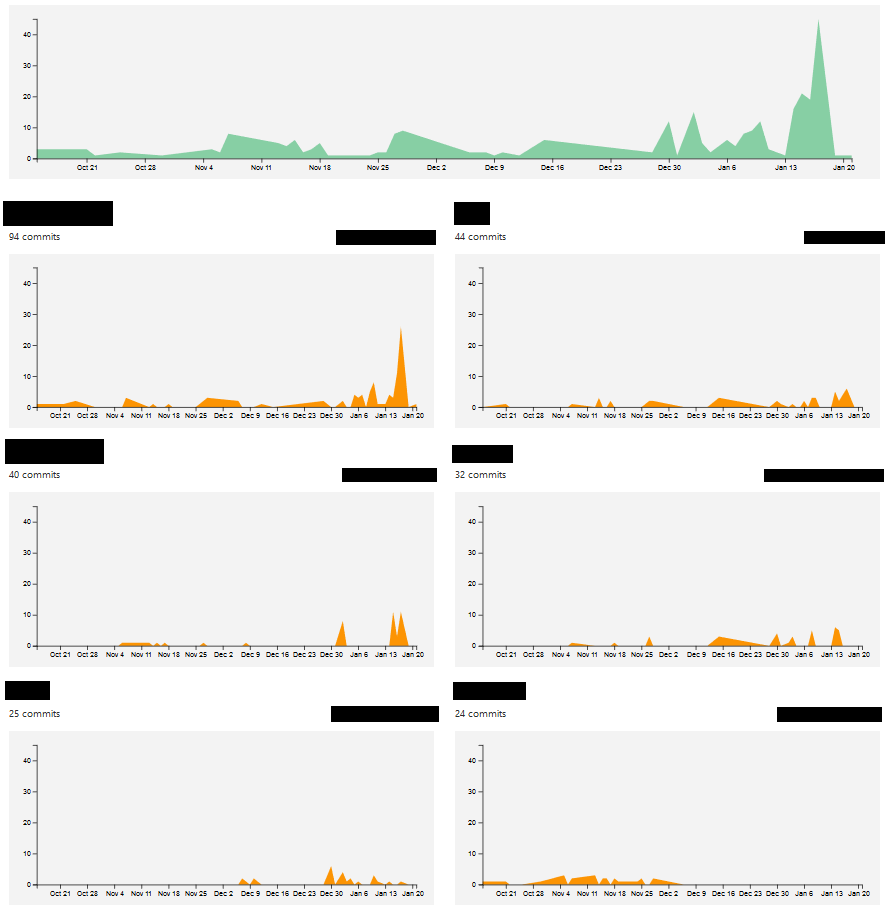
\includegraphics[scale=0.4]{slike/aktivnost.PNG}
	\centering
	\caption{Primjer slike s potpisom}
	\label{fig:promjene}
\end{figure}

\begin{figure}[H]
	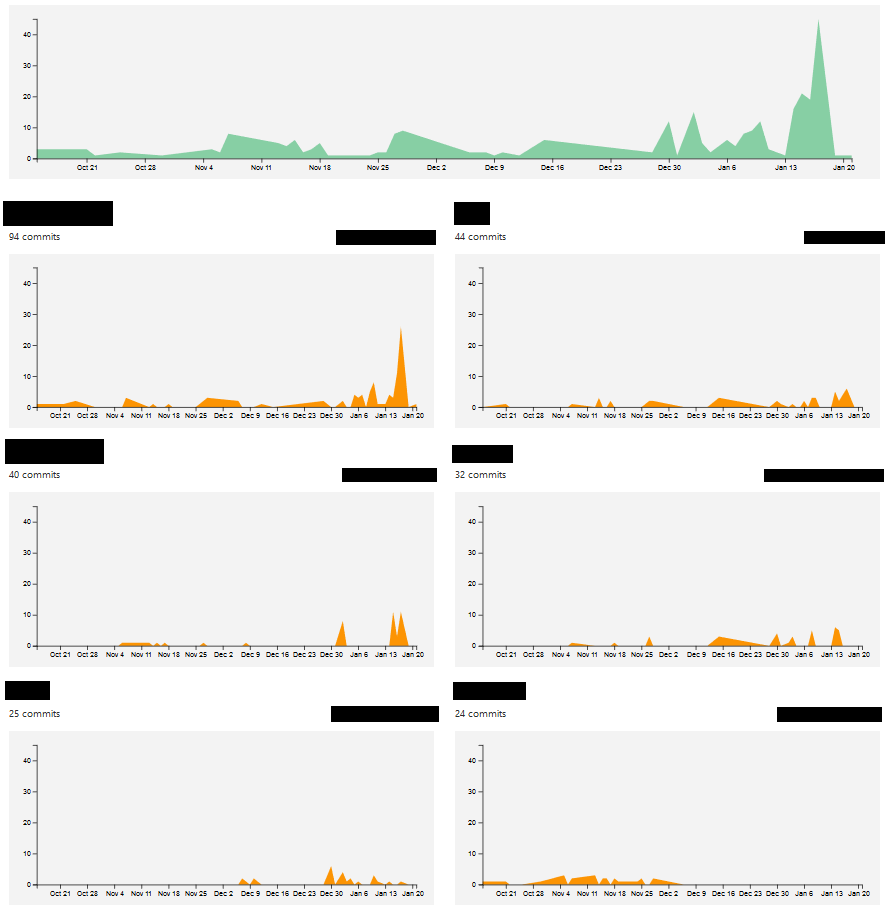
\includegraphics[width=\linewidth]{slike/aktivnost.PNG}
	\caption{Primjer slike s potpisom 2}
	\label{fig:promjene2}
\end{figure}



\eject

